%%%%%%%%%%%%%%%%%%%%%%%%%%%%%%%%%%%%%%%%%%%%%%%%%%%%%%%%%%%%%%%%%%%%%%
% Lớp 10 | Hệ thức lượng trong tam giác | Định lý sin và định lý côsin
% Dạng 0H4?2-1: Bài toán chỉ dùng định lý Sin, Côsin
% Số câu: 64  (sinh tự động bởi tach_cau.py; từ nay thầy sửa trực tiếp file này)
%%%%%%%%%%%%%%%%%%%%%%%%%%%%%%%%%%%%%%%%%%%%%%%%%%%%%%%%%%%%%%%%%%%%%%

%%%%%%%%%%%%%%%% TRẮC NGHIỆM 4 PHƯƠNG ÁN %%%%%%%%%%%%%%%%

% nguồn: MaHoaNH_TracNghiem_Lop10
\begin{ex}%[0H4N2-1]%[ma:406d4f4b]
	 Cho $\triangle ABC$ có $b=6$, $c=8$, $\hat{A}=120^{\circ}$. Tính độ dài cạnh $a$.
	 \choice {\True $2\sqrt{37}$}{$3\sqrt{12}$}{$2\sqrt{13}$}{$\sqrt{20}$}
	\loigiai{ 
		 $a^{2}=b^{2}+c^{2}-2bc\cos A=6^{2}+8^{2}-2\cdot6\cdot8\cdot\cos 120^{\circ}=148$.\\
		 $a=2\sqrt{37}$.
	} 
\end{ex}

% nguồn: MaHoaNH_TracNghiem_Lop10
\begin{ex}%[0H4N2-1]%[ma:9295f360]
	Cho tam giác  $ABC$, biết $AB=4$, $AC=5$, $BC=\sqrt{21}$. Tính góc $\widehat{BAC}$ của tam giác $ABC$?
	\choice {$\widehat{BAC}=120^{\circ}$}{\True $\widehat{BAC}=60^{\circ}$}{$\widehat{BAC}=150^{\circ}$}{$\widehat{BAC}=90^{\circ}$} 
	 \loigiai{
		Áp  dụng định lí côsin\\
		 $\cos\widehat{BAC}=\dfrac{AB^{2}+AC^{2}-BC^{2}}{2.AB.AC}=\dfrac{4^{2}+5^{2}-(\sqrt{21})^{2}}{2\cdot4\cdot5}=\dfrac{16+25-21}{40}=\dfrac{20}{40}=\dfrac{1}{2}$.\\
		Suy ra $\widehat{BAC}=60^{\circ}$. 
	 }
\end{ex}

% nguồn: MaHoaNH_TracNghiem_Lop10
\begin{ex}%[0H4N2-1]%[ma:567b4459]
	Cho tam giác $ABC$ có  ba cạnh $a=5$, $b=6$, $c=7$. Tính côsin góc $A$.
	 \choice
		{\True  $\dfrac{5}{7}$}
		 {$\dfrac{2}{21}$}
		 {$\dfrac{55}{42}$}
		 {$\dfrac{10}{7}$}
	 \loigiai{
	Áp dụng định lí côsintrong tam giác  ta có $\cos A=\dfrac{b^2+c^2-a^2}{2bc}=\dfrac{5}{7}$.}
\end{ex}

% nguồn: MaHoaNH_TracNghiem_Lop10
\begin{ex}%[0H4N2-1]%[ma:a2035388]
	Cho tam giác $ABC$ có $AB=c$, $BC=a$, $AC=b$. Hãy chọn mệnh đề  \textbf{sai} trong các mệnh đề sau?
	 \choice
		 {$\cos A=\dfrac{b^2+c^2-a^2}{2bc}$}
		{$b\cdot\sin C=c\cdot\sin  B$}
		{$\dfrac{a}{\sin A}=2R$} 
		{\True $b^2=a^2+c^2+2ac\cdot\cos B$} 
	 \loigiai{
	Ta có $b^2=a^2+c^2-2ac\cdot\cos  B$.}
\end{ex}

% nguồn: MaHoaNH_TracNghiem_Lop10
\begin{ex}%[0H4N2-1]%[ma:e166c3ad]
	Tam giác $ABC$ có $BC=a$; $AB=c$; $AC=b$ và  có $R$ là bán kính đường tròn ngoại tiếp. Hệ thức nào sau đây là đúng?
	\choice 
		{$\sin C=\dfrac{a \cdot \sin A}{c}$} 
		 {\True $\dfrac{b}{\sin B}=2 R$}
		{$\sin A=\dfrac{2a}{R}$} 
		{$\dfrac{a}{\sin A}=\dfrac{2}{3}$} 
	\loigiai{ 
	Theo lý thuyết ta có $\dfrac{a}{\sin A}=\dfrac{b}{\sin B}=\dfrac{c}{\sin  C}=2 R$.}
\end{ex}

% nguồn: MaHoaNH_TracNghiem_Lop10
\begin{ex}%[0H4N2-1]%[ma:7451eb3b]
	Cho tam giác $ABC$, biết $AB=3$, $AC=5$,  $BC=7$. Tính góc $\widehat{BAC}$ của tam giác $ABC$?
	\choice  {\True$\widehat{BAC}=120^{\circ}$}{$\widehat{BAC}=60^{\circ}$}{$\widehat{BAC}=150^{\circ}$}{$\widehat{BAC}=90^{\circ}$}
	\loigiai{ 
		Áp dụng định lý  côsintrong $\Delta ABC$, ta có\\
		$BC^{2}=AB^{2}+AC^{2}-2.AB.AC.\cos\widehat{BAC}$\\ 
		 $\Rightarrow \cos\widehat{BAC}=\dfrac{AB^{2}+AC^{2}-BC^{2}}{2.AB.AC}=\dfrac{3^2+5^2-7^2}{2\cdot3\cdot5}=\dfrac{9+25-49}{30}=\dfrac{-15}{30}=-\dfrac{1}{2}.$\\
		Suy  ra $\widehat{BAC}=120^{\circ}$.
	 }
\end{ex}

% nguồn: MaHoaNH_TracNghiem_Lop10
\begin{ex}%[0H4N2-1]%[ma:5c9dbf45]
	Cho tam  giác $ABC$ có $a=4$, $b=3$, $\widehat C=60^\circ$. Tính độ dài cạnh $c$.
	\choice 
		 {\True $c=\sqrt{13}$}
		 {$c=13$}
		 {$c=5$}
		{$c=\sqrt{25+12\sqrt  3}$}
	 \loigiai{
		Theo định lý côsinta có $c^2=a^2+b^2-2ab\cos\widehat  C=4^2+3^2-2\cdot4\cdot3\cdot\dfrac{1}{2}=13\Rightarrow c=\sqrt{13}$.
	 }
\end{ex}

% nguồn: MaHoaNH_TracNghiem_Lop10
\begin{ex}%[0H4N2-1]%[ma:b34528f9]
	 Gọi $R$ là bán kính đường tròn ngoại tiếp tam giác $ABC$. Đẳng thức nào dưới đây \textbf{sai}?
	\choice 
		 {$\dfrac{a}{\sin A}=2R$}
		 {$\sin A=\dfrac{a}{2R}$}
		{\True $b\sin B=2R$} 
		{$\sin C=\dfrac{c\sin A}{a} $} 
	\loigiai{ 
		Từ định lý hàm số sintrong tam giác  $ABC$ ta có $\dfrac{a}{\sin A}=\dfrac{b}{\sin B}=\dfrac{c}{\sin C}=2R$.
	} 
\end{ex}

% nguồn: MaHoaNH_TracNghiem_Lop10
\begin{ex}%[0H4N2-1]%[ma:f64de051]
	Cho tam giác $ABC$ với $BC=a, CA=b, AB=c$, $S$ là diện tích tam giác và $R$ là bán kính đường tròn ngoại tiếp  tam giác $ABC$. Khẳng định nào sau đây đúng?
	 \choice
		{$\dfrac{a}{\sin  A}=\dfrac{b}{\sin B}=\dfrac{c}{\sin C}=R$}
		 {$a^2=b^2+c^2+2bc\cos A$}
		{$S=\dfrac{1}{2}ab\cos  C$}
		{\True $\dfrac{a}{\sin A}=\dfrac{b}{\sin B}=\dfrac{c}{\sin  C}=2R$}
	 \loigiai{
		Theo  định lý Sin, $\dfrac{a}{\sin A}=\dfrac{b}{\sin B}=\dfrac{c}{\sin C}=2R$.
	} 
\end{ex}

% nguồn: MaHoaNH_TracNghiem_Lop10
\begin{ex}%[0H4N2-1]%[ma:cc707a8b]
	Cho $\triangle ABC$ có $AB=4$, $AC=6$,  $\widehat{A}=120^\circ $. Độ dài cạnh $BC$ là
	\choice 
		 {$\sqrt{19}$}
		{$3\sqrt{19}$} 
		{\True $2\sqrt{19}$} 
		 {$2\sqrt{7}$}
	 \loigiai{
		Áp dụng Định lí Côsinta có 
		$$BC^2=AB^2+AC^2-2\cdot AB\cdot  AC\cdot \cos A
	 \Rightarrow BC=\sqrt{4^2+6^2-2\cdot 4\cdot 6\cdot \cos 120^\circ}=2\sqrt{19}.$$}
\end{ex}

% nguồn: MaHoaNH_TracNghiem_Lop10
\begin{ex}%[0H4N2-1]%[ma:ce10d6a0]
	Cho tam giác $ABC$ có $AB=5$, $BC=7$, $CA=8$. Số đo  góc $A$ bằng
	 \choice
		{$45^\circ $} 
		 {$90^\circ $}
		{\True $60^\circ  $}
		{$30^\circ $} 
	 \loigiai{
		Ta có $\cos\widehat{BAC}=\dfrac{AB^2+AC^2-BC^2}{2AB\cdot  AC}=\dfrac{1}{2}\Rightarrow\widehat{BAC}=60^\circ $.\\
		Vậy số  đo góc $A$ bằng $60^\circ $.
	 }
\end{ex}

% nguồn: MaHoaNH_TracNghiem_Lop10
\begin{ex}%[0H4N2-1]%[ma:f4da0382]
	Cho tam giác $ABC$ có $AB=7$ cm,  $AC=3$ cm và $\widehat{A}=60^\circ$. Tính độ dài cạnh $BC$.
	 \choice
		{$BC=5{,}58$} 
		 {$BC=9{,}08$}
		{$BC=7{,}08$} 
		 {\True $BC=6{,}08$}
	\loigiai{ 
		 Áp dụng Định lí cô-sintrong tam giác $ABC$ ta có
		$$BC^2=AB^2+AC^2-2AB \cdot AC \cdot \cos A=49+9-2\cdot 7\cdot  3\cdot \dfrac{1}{2}=37.$$
		Do đó,  $BC=\sqrt{37}=6{,}08$ cm.
	 }
\end{ex}

% nguồn: MaHoaNH_TracNghiem_Lop10
\begin{ex}%[0H4H2-1]%[ma:d160142b]
	 Cho tam giác $ABC$ thoả mãn $b^2+c^2-a^2=\sqrt{2}bc$. Khi đó
	\choice  {$A=30^\circ$}{\True $A=45^\circ$}{$A=60^\circ$}{$A=75^\circ$}
	\loigiai{ 
		$\cos A=\dfrac{b^2+c^2-a^2}{2bc}=\dfrac{\sqrt{2}bc}{2bc}=\dfrac{\sqrt{2}}{2}\Rightarrow\widehat{A}=45^\circ$. 
	 }
\end{ex}

% nguồn: MaHoaNH_TracNghiem_Lop10
\begin{ex}%[0H4H2-1]%[ma:eecf9ad0]
	Cho tam giác $ABC$ có $AB=5$; $BC=7$; $AC=8$.  Số đo góc $A$ bằng
	\choice { $45^{\circ}$}{ $90^{\circ}$}{\True $60^{\circ}$}{ $30^{\circ}$} 
	 \loigiai{
		Theo hệ quả  định lý côsinta có
		$\cos  A=\dfrac{AB^{2}+AC^{2}-BC^{2}}{2AB\cdot AC}=\dfrac{5^{2}+8^{2}-7^{2}}{2\cdot5\cdot8}=\dfrac{1}{2}$
		Suy ra  $A=60^{\circ}$.
	} 
\end{ex}

% nguồn: MaHoaNH_TracNghiem_Lop10
\begin{ex}%[0H4H2-1]%[ma:8c3a5f59]
	Cho tam giác $ABC$  có $\widehat{A}=120^{\circ}$. Hệ thức nào sau đây đúng?
	 \choice {\True $a^{2}=b^{2}+c^{2}+bc$}{$a^{2}=b^{2}+c^{2}-3bc$}{$a^{2}=b^{2}+c^{2}-bc$}{$a^{2}=b^{2}+c^{2}+3bc$}
	\loigiai{ 
		 Áp dụng Định lí côsin
		$a^{2}=b^{2}+c^{2}-2bc\cdot\cos A$.\\ 
		 Với $A=120^{\circ}$ thì $\cos A=\cos 120^{\circ}=-\dfrac{1}{2}$.\\
		$a^{2}=b^{2}+c^{2}-2bc\cdot\left(-\dfrac{1}{2}\right)=b^{2}+c^{2}+bc$. 
	 }
\end{ex}

% nguồn: MaHoaNH_TracNghiem_Lop10
\begin{ex}%[0H4H2-1]%[ma:83d734b5]
	Cho tam  giác $ABC$ có $b^2+c^2-a^2< 0$. Kết luận nào sau đây đúng?
	 \choice
		{$\widehat{A} <  90^\circ$}
		{\True $90^\circ  < \widehat{A} < 180^\circ$}
		{$90^\circ < \widehat{B} < 180^\circ$} 
		{$90^\circ < \widehat{C} < 180^\circ$} 
	 \loigiai{
	Ta có $\cos A=\dfrac{b^2+c^2-a^2}{2bc}< 0\Rightarrow  90^\circ < \widehat{A} < 180^\circ$.}
\end{ex}

% nguồn: MaHoaNH_TracNghiem_Lop10
\begin{ex}%[0H4H2-1]%[ma:c04a870b]
	Cho tam giác $ABC$ có $\widehat{BAC}=60^\circ$, $\widehat{ABC}=45^\circ$, $BC=\sqrt{6} $\,m. Độ dài cạnh  $AC$ bằng
	 \choice
		{$4$\,m} 
		 {$\sqrt{2}$\,m}
		 {\True $2$\,m}
		{$1$\,m} 
	 \loigiai{
		Áp đụng định lí sinta có $\dfrac{BC}{\sin A}=\dfrac{AC}{\sin B}\Rightarrow AC=\dfrac{BC\cdot  \sin B}{\sin A}=\dfrac{\sqrt{6}\sin45^\circ}{\sin60^\circ}=2$\,m.
	} 
\end{ex}

% nguồn: MaHoaNH_TracNghiem_Lop10
\begin{ex}%[0H4H2-1]%[0H4H2-1]%[ma:9fce14f5]
	Cho tam giác $ABC$ thỏa  mãn hệ thức $b+c=2a$. Mệnh đề nào sau đây là đúng?
	\choice 
		{$\cos B+\cos C=2\cos A$} 
		 {\True $\sin B+\sin C=2\sin A$}
		{$\sin B+\sin C=\dfrac{1}{2}\sin A$} 
		 {$\sin B+\cos C=2\sin A$}
	\loigiai{ 
		Ta có $b+c=2a$ $\Leftrightarrow 2R\sin B+2R\sin C=2\cdot 2R\sin  A$ $\Leftrightarrow\sin B+\sin C=2\sin A$.
	} 
\end{ex}

% nguồn: MaHoaNH_TracNghiem_Lop10
\begin{ex}%[0H4H2-1]%[ma:408a4c73]
	 Cho tam giác $ABC$ có $BC=10$ và góc $A=30^\circ$. Bán kính $R$ của đường tròn ngoại tiếp tam giác $ABC$ bằng
	 \choice
		{$\dfrac{10}{\sqrt  3}$}
		{$5$} 
		{$10\sqrt 3 $} 
		 {\True $10$}
	 \loigiai{
		Áp dụng định lý sintrong tam giác $ABC$ ta có $$2R=\dfrac{BC}{\sin A}=\dfrac{10}{\sin  30^\circ}=\dfrac{10}{\dfrac{1}{2}}\Rightarrow R=10.$$
	 }
\end{ex}

% nguồn: MaHoaNH_TracNghiem_Lop10
\begin{ex}%[0H4H2-1]%[ma:115f7ea6]
	 Cho tam giác $ABC$ có $AB=5$, $BC=7$, $AC=8$. Số đo góc $A$ bằng
	\choice 
		{$45^\circ$} 
		 {$90^\circ$}
		{\True $60^\circ$} 
		{$30^\circ$} 
	\loigiai{ 
		Ta có  $AB=5$, $BC=7$, $AC=8$.\\
	Từ đó suy  ra $\cos A=\dfrac{AC^2+AB^2-BC^2}{2AB\cdot AC}=\dfrac{8^2+5^2-7^2}{2\cdot 8\cdot 5}=\dfrac{1}{2}\Rightarrow \widehat{A}=60^\circ$.}
\end{ex}

% nguồn: MaHoaNH_TracNghiem_Lop10
\begin{ex}%[0H4H2-1]%[ma:b722c837]
	Cho $\triangle ABC$ có $AB=5$, $\widehat{A}=40^\circ$,  $\widehat{B}=60^\circ$. Độ dài $BC$ gần nhất với kết quả nào?
	\choice 
		 {$3{,}7$}
		{\True  $3{,}3$}
		{$3{,}5$} 
		{$3{,}1$} 
	\loigiai{ 
		Ta có  $\widehat{C}=180^\circ-\widehat{A}-\widehat{B}=180^\circ-40^\circ-60^\circ=80^\circ$.\\
	Áp dụng định lý sin: $\dfrac{BC}{\sin A}=\dfrac{AB}{\sin C}\Rightarrow BC=\dfrac{AB}{\sin C}\cdot\sin  A=\dfrac{5}{\sin 80^\circ}\cdot\sin 40^\circ\approx 3{,}3$.}
\end{ex}

% nguồn: MaHoaNH_TracNghiem_Lop10
\begin{ex}%[0H4H2-1]%[ma:07d31826]
	Cho tam giác $ABC$ nhọn có $BC=3a$ và bán kính đường tròn ngoại tiếp tam giác $ABC$ là  $R=a\sqrt 3 $. Tính số đo góc $A$.
	 \choice
		{$\widehat{A}=45^\circ $} 
		 {$\widehat{A}=30^\circ $}
		{\True $\widehat{A}=60^\circ $} 
		 {$\widehat{A}=120^\circ $}
	\loigiai{ 
		Áp dụng định lý sintrong tam giác $ABC$,  ta có $$\dfrac{BC}{\sin A}=2R\Rightarrow\sin A=\dfrac{BC}{2R}=\dfrac{3a}{2a\sqrt 3}=\dfrac{\sqrt 3}{2}.$$
		Suy  ra $\widehat{A}=60^\circ $ (do tam giác $ABC$ nhọn).
	 }
\end{ex}

% nguồn: MaHoaNH_TracNghiem_Lop10
\begin{ex}%[0H4H2-1]%[ma:f0d7991d]
	Tam giác ABC có $\widehat A=68^\circ 12'$, $\widehat  B=34^\circ 44'$, $AB=117$. Tính $AC$.
	\choice 
		{\True $68$} 
		 {$168$}
		{$118$} 
		{$200$} 
	\loigiai{ 
		Ta  có trong tam giác $ABC$: $\widehat A+\widehat B+\widehat C=180^\circ\Rightarrow\widehat C=180^\circ-68^\circ12'-34^\circ44'=77^\circ4'$.\\
		 Mặt khác $$\dfrac{a}{\sin A}=\dfrac{b}{\sin B}=\dfrac{c}{\sin C}\Rightarrow\dfrac{AC}{\sin B}=\dfrac{AB}{\sin C}\Rightarrow AC=\dfrac{AB\cdot\sin B}{\sin C}=\dfrac{117\cdot\sin{34^\circ}44'}{\sin77^\circ4'}\approx 68.$$
	} 
\end{ex}

% nguồn: MaHoaNH_TracNghiem_Lop10
\begin{ex}%[0H4H2-1]%[ma:776469cf]
	Cho $\triangle ABC$ có $AB=5$, $\widehat{A}=40^\circ$, $\widehat{B}=60^\circ $. Độ dài  $BC$ gần nhất với kết quả nào?
	 \choice
		 {\True $3{,}1$}
		{$3{,}7$} 
		{$3{,}5$} 
		{$3{,}8$} 
	\loigiai{ Ta có $\widehat{C}=180^\circ-\left(40^\circ+60^\circ\right)=80^\circ$. \\ 
		Áp đụng định lý sin vào $\triangle  ABC$\\
		$\dfrac{AB}{\sin C}=\dfrac{BC}{\sin  A}\Rightarrow BC=\dfrac{AB}{\sin C}\cdot\sin A=\dfrac{5}{\sin 80^\circ}\cdot\sin 40^\circ\approx 3{,}26$.
	} 
\end{ex}

% nguồn: MaHoaNH_TracNghiem_Lop10
\begin{ex}%[0H4H2-1]%[ma:263fe750]
	Tam giác $ABC$ có $\widehat{B}=60^\circ, \widehat{C}=45^\circ, AB=5$ hỏi cạnh $BC$ gần với số  nào nhất?
	\choice 
		{\True $6{,}83$} 
		{$6{,}84$} 
		 {$6{,}82$}
		{$6{,}81$} 
	 \loigiai{
		Ta  có $\widehat{A}=180^\circ-\widehat{B}-\widehat{C}=180^\circ-60^\circ-45^\circ=75^\circ$.\\
		 Áp dụng định lí sin vào tam giác $ABC$ ta được
	\[\dfrac{BC}{\sin A}=\dfrac{AB}{\sin C}\Rightarrow BC=AB\cdot\dfrac{\sin  A}{\sin C}\approx 6{,}83.\]}
\end{ex}

% nguồn: MaHoaNH_TracNghiem_Lop10
\begin{ex}%[0H4H2-1]%[ma:17a9876c]
	Cho tam giác $ABC$ có $\dfrac{5}{\sin A}=\dfrac{4}{\sin B}=\dfrac{3}{\sin C}$ và $a=10$.  Tính chu vi tam giác đó.
	 \choice
		{\True $24$} 
		 {$36$}
		 {$22$}
		 {$12$}
	\loigiai{ 
		Ta  có $\dfrac{5}{\sin A}=\dfrac{4}{\sin B}=\dfrac{3}{\sin C}\Leftrightarrow\dfrac{10}{\sin A}=\dfrac{8}{\sin B}=\dfrac{6}{\sin C}\Leftrightarrow\dfrac{a}{\sin A}=\dfrac{8}{\sin B}=\dfrac{6}{\sin C}$.\\
		Theo định lý sintrong  tam giác ta tính được $b=8$, $c=6$.\\
		Chu vi tam  giác là $a+b+c=24$.
	 }
\end{ex}

% nguồn: MaHoaNH_TracNghiem_Lop10
\begin{ex}%[0H4H2-1]%[ma:924993a8]
	Tính chu vi tam giác  $ABC$ biết rằng $AB=6$ và $2\sin A=3\sin B=4\sin C$.
	\choice 
		{$10\sqrt 6$} 
		 {\True $26$}
		{$13$} 
		{$5\sqrt{26}$} 
	 \loigiai{
		Ta có $\dfrac{AB}{\sin C}=\dfrac{AC}{\sin B}\Rightarrow\dfrac{6}{\dfrac{3}{4}\sin  B}=\dfrac{AC}{\sin B}\Rightarrow AC=8$.\\
		Và $\dfrac{BC}{\sin  A}=\dfrac{AC}{\sin B}\Rightarrow\dfrac{BC}{\sin A}=\dfrac{8}{\dfrac{2}{3}\sin A}\Rightarrow BC=12$.\\
		Chu vi tam  giác $C=AB+BC+CA=26$.
	 }
\end{ex}

% nguồn: MaHoaNH_TracNghiem_Lop10
\begin{ex}%[0H4H2-1]%[ma:97507779]
	\immini[thm]{Khoảng cách từ $A$ đến $B$  không thể đo trực tiếp được vì phải đi qua một đầm lầy. Người ta xác định một điểm $C$ mà từ đó có thể nhìn được $A$ và $B$ dưới một góc $78^\circ 24'$. Biết rằng $CA=250$\,m, $CB=120$\,m. Khoảng cách $AB$ bằng bao nhiêu?
	\choice 
		{\True $255$\,m} 
		 {$166$\,m}
		 {$298$\,m}
		 {$266$\,m}}
		{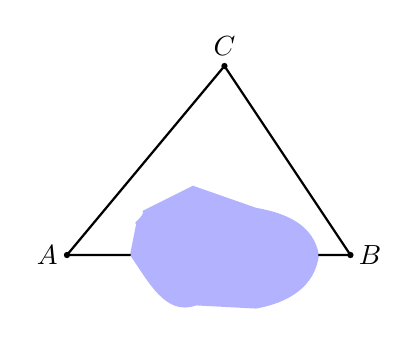
\begin{tikzpicture}[line join=round,line cap=round,>=stealth,thick,scale=0.8]
		\fill[blue!30]  (0,0)
			to[out=-55,in=200] (1.05,-0.8)--(2,-.85) 
			 to[out=10,in=263] (3,0)
			to[out=100,in=-10] (2,0.75)--(1,1.1)--(0.2,0.7) 
			 to[out=-55,in=190] (.1,0.5)--cycle;
		 \path
			(-1,0) coordinate  (A)
			 (1.5,3) coordinate (C)
			(3.5,0)  coordinate (B);
		\draw  [thick] (0,0)--(A)--(C)--(B)--(3,0);
		\foreach \i/\g in {C/90,A/180,B/0} \fill (\i) circle (.05)  node[shift={(\g:.25)}] {$\i$};
	\end{tikzpicture}
		 }
	\loigiai{ 
	Ta  có $AB=\sqrt{AC^2+BC^2-2AC\cdot BC\cdot\cos \widehat{ACB}}\approx 255$\,m.}
\end{ex}

% nguồn: MaHoaNH_TracNghiem_Lop10
\begin{ex}%[0H4Y2-1]%[ma:3be55adc]
	Trong mặt phẳng $O x y$, toạ độ tâm của đường tròn  $(\mathscr{C})\colon(x-2)^2+(y+3)^2=4$ là
	 \choice
		{$(-2;  3)$}
		{$(-3; 2)$} 
		 {$(3;-2)$}
		{\True$(2;-3)$} 
	\loigiai{Toạ độ tâm của đường tròn $(\mathscr{C})\colon(x-2)^2+(y+3)^2=4$ là $(2;-3)$.} 
\end{ex}

% nguồn: MaHoaNH_TracNghiem_Lop10
\begin{ex}%[0H4Y2-1]%[ma:0e4054d9]
	Cho  đường tròng $\left(C\right)$ có phương trình$\colon\left(x-3\right)^2+\left(y+2\right)^2=25$. Toạ độ tâm $I$ và bán kính $R$ của đường tròn là?
	\choice 
		 {$I\left(2;-3\right)$ và $R=5$}
		{$I\left(-3;2\right)$ và $R=5$} 
		 {\True $I\left(3;-2\right)$ và $R=5$}
		 {$I\left(3;-2\right)$ và $R=25$}
	\loigiai{Toạ độ tâm $I$ và bán kính $R$ của đường  tròn là$\colon I\left(3;-2\right)$ và $R=5$
	 }
\end{ex}

% nguồn: MaHoaNH_TracNghiem_Lop10
\begin{ex}%[0H4Y2-1]%[ma:e2432a9e]
	Cho đường tròn $(C)$ có phương trình: $\left(x-1\right)^2+\left(y-2\right)^2=9$. Tìm tọa độ tâm và bán kính của đường  tròn $(C)$.
	\choice 
		{\True  Đường tròn $(C)$ có tâm $ I\left(1;2\right)$ và bán kính $ R=3$}
		{Đường  tròn $(C)$ có tâm $ I\left(-1;-2\right)$ và bán kính $ R=9$}
		{Đường tròn $(C)$ có tâm $ I\left(1;2\right)$  và bán kính $ R=9$}
		{Đường tròn $(C)$ có tâm $ I\left(-1;-2\right)$ và bán kính $  R=3$}
	 \loigiai{
	Đường tròn $(C)$ có tâm $ I\left(1;2\right)$ và bán kính $ R=3$.} 
\end{ex}

% nguồn: MaHoaNH_TracNghiem_Lop10
\begin{ex}%[0H4K2-1]%[ma:c2495e8a]
	Trong mặt phẳng $O x y$, cho tam giác $O A B$ có $O(0; 0), A(6; 0), B(0; 8)$. Gọi $M, N, P$ lần  lượt là trung điểm của các cạnh $O A, O B, A B$. Đường tròn đi qua ba điểm $M, N, P$ có bán kính là
	 \choice
		{\True  $\dfrac{5}{2}$}
		{$ 5 $} 
		{$5 \sqrt{2}$} 
		{$  10 $}
	\loigiai{Ta có $M, N, P$ lần lượt là trung điểm của các cạnh $O  A, O B, A B$ nên $ M(3;0), N(0;4), P(3;4) $. \\
	Khi đó, $ \overrightarrow{NP}\cdot\overrightarrow{MP}=0 $. Suy ra $ \triangle MNP $ vuông tại $ P $.\\ Vậy bán kính đường tròn ngoại tiếp $  \triangle MNP $ là $ \dfrac{MN}{2}=\dfrac{5}{2} $.}
\end{ex}

% nguồn: MaHoaNH_TracNghiem_Lop10
\begin{ex}%[0H4Y2-1]%[ma:6f6727d1]
	Trong mặt phẳng tọa độ $Oxy$, cho đường tròn $(C)\colon  x^2+y^2-4x+2y+1=0$. Tâm $I$ của $(C)$ có tọa độ là
	 \choice
		 {$I(-2; 1)$}
		{$I(4;-2)$} 
		{$I(-4; 2)$} 
		{\True  $I(2;-1)$}
	\loigiai{ 
		 Tâm $I$ của $(C)$ có tọa độ là $(2;-1)$.
	} 
\end{ex}

% nguồn: MaHoaNH_TracNghiem_Lop10
\begin{ex}%[0H4Y2-1]%[ma:6e386a0b]
	Đường  tròn $(C)\colon (x+1)^2+(y+2)^2=9$ có tâm $I$ là
	 \choice
		{\True  $I(-1;-2)$}
		 {$I(1;-2)$}
		 {$I(1; 2)$}
		{$I(-1;  2)$}
	\loigiai{ 
		Đường  tròn $ (C) $ có tâm $ I(-1;-2) $.
	 }
\end{ex}

% nguồn: MaHoaNH_TracNghiem_Lop10
\begin{ex}%[0H4Y2-1]%[ma:ee377ad3]
	Trong mặt phẳng tọa độ $Oxy$, đường tròn $(C) \colon x^2+y^2+4x+6y-12=0$ có tâm  là
	 \choice
		{\True  $I(-2;-3)$}
		{$I(2;3)$} 
		{$I(4;6)$} 
		 {$I(-4;-6)$}
	 \loigiai{
		Tâm của đường tròn $(C)$ là $I(-2;-3)$. 
	 }
\end{ex}

% nguồn: MaHoaNH_TracNghiem_Lop10
\begin{ex}%[0H4Y2-1]%[ma:7e0d31af]
	Trong mặt phẳng với hệ trục $Oxy$ cho đường tròn $(C)\colon  (x-2)^2 +(y+ 4)^2=16$. Đường tròn $(C)$ có toạ độ tâm $I$ và bán kính $R$ bằng
	\choice 
		 {\True $I(2;-4)$, $R=4$}
		{$I(2;-4)$, $R=16$} 
		 {$I(-2;4)$, $R=4$}
		 {$I(-2;4)$, $R=16$}
	\loigiai{ 
		Đường tròn $(C)$ có toạ độ tâm $I$ và  bán kính $R$ bằng $I(2;-4)$, $R=4$.
	} 
\end{ex}

% nguồn: MaHoaNH_TracNghiem_Lop10
\begin{ex}%[0H4Y2-1]%[ma:b33f84af]
	Đường tròn $x^2+y^2-6 x-8 y=0$  có bán kính bằng bao nhiêu?
	\choice 
		{$ 25  $}
		 {\True $ 5 $}
		{$\sqrt{10}$} 
		 {$ 10 $}
	\loigiai{ 
		Ta có $x^2+y^2-6 x-8 y=0\Leftrightarrow (x-3)^2+(y-4)^2=25$. Do đó bán kính đường tròn là $ R=5  $.
	} 
\end{ex}

% nguồn: MaHoaNH_TracNghiem_Lop10
\begin{ex}%[0H4B2-1]%[ma:01548f3f]
	Trong mặt phẳng tọa độ $Oxy$, cho đường tròn $(C)\colon (x-1)^2+(y+3)^2=16$. Tọa độ tâm  $I$ của đường tròn $(C)$ là
	\choice 
		{\True $(1;-3)$} 
		{$(-3;1)$} 
		{$(-1;-3)$} 
		{$(1;3)$} 
	 \loigiai{
		Tọa độ tâm $I$  của đường tròn $(C)$ là $(1;-3)$
	} 
\end{ex}

% nguồn: MaHoaNH_TracNghiem_Lop10
\begin{ex}%[0H4Y2-1]%[ma:969a3ae9]
	Trong mặt phẳng $Oxy$, cho  đường tròn có phương trình $(C)\colon (x-1)^2+(y+3)^2=16$. Tọa độ tâm $I$ và bán kính $R$ của đường tròn $(C)$ là
	\choice 
		{\True $I(1;-3)$,  $R=4$}
		 {$I(1;-3)$, $R=16$}
		{$I(-1;3)$, $R=16$} 
		 {$I(-1;3)$, $R=4$}
	\loigiai{ 
		Đường tròn $(C)\colon  (x-1)^2+(y+3)^2=16$ có tâm $I(1;-3)$ và bán kính $R=\sqrt{16}=4$.
	} 
\end{ex}

% nguồn: MaHoaNH_TracNghiem_Lop10
\begin{ex}%[0H4Y2-1]%[ma:ba289d7a]
	Tìm tọa độ tâm  $I$ và bán kính $R$ của đường tròn $(C)\colon x^2+y^2-2x+4y+1=0$.
	 \choice
		{$I(-1;2)$; $R=\sqrt{5}$} 
		{\True $I(1;-2)$; $R=2$} 
		{$I(1;-2)$;  $R=4$}
		 {$I(-1;2)$; $R=4$}
	\loigiai{ 
	Đường tròn $(C)$ có tâm $I(1;-2)$ và  bán kính $R=\sqrt{1^2+\left(-2\right)^2-1}=2$.
	} 
\end{ex}

% nguồn: MaHoaNH_TracNghiem_Lop10
\begin{ex}%[0H4B2-1]%[ma:1cf2a8e3]
	Trong mặt phẳng $Oxy$, cho đường tròn $(C)\colon x^2+y^2+4x-6y-3=0$. Tìm toạ độ tâm $I$ và tính bán  kính $R$ của $(C)$.
	\choice 
		{$I(-2;3)$, $R=16$} 
		 {\True $I(-2;3)$, $R=4$}
		 {$I(2;-3)$, $R=15$}
		{$I(2;-3)$, $R=4$} 
	\loigiai{ 
		Đường tròn $(C)$ có  tâm $I(-2;3)$, bán kính $R=\sqrt{(-2)^2+3^2-(-3)}=4$.
	 }
\end{ex}

% nguồn: MaHoaNH_TracNghiem_Lop10
\begin{ex}%[0H4Y2-1]%[ma:f4dd8758]
	Trong mặt  phẳng tọa độ $Oxy$, tọa độ tâm $I$ và bán kính $R$ của đường tròn $(C)$ có phương trình $(x+2)^2+(y-4)^2=9$ là
	\choice 
		 {$I(2;-4)$, $R=3$}
		{$I(-1;2)$, $R=3$} 
		 {$I(1;-2)$, $R=3$}
		{\True  $I(-2;4)$, $R=3$}
	 \loigiai{
		Đường tròn $(C)$ có tâm $I(-2;4)$, bán kính $R=3$. 
	 }
\end{ex}

% nguồn: MaHoaNH_TracNghiem_Lop10
\begin{ex}%[0H4B2-1]%[ma:01456dd8]
	Trong mặt phẳng $Oxy$, đường tròn $(C)\colon  x^2+y^2+4x+6y-12=0$ có tâm là
	\choice 
		{$I(2;3)$} 
		{\True  $I(-2;-3)$}
		 {$I(-4;-6)$}
		 {$I(4;6)$}
	 \loigiai{
		Đường tròn $(C)\colon  x^2+y^2+4x+6y-12=0$ có tâm $I(-2;-3)$.
	 }
\end{ex}

% nguồn: MaHoaNH_TracNghiem_Lop10
\begin{ex}%[0H4Y2-1]%[ma:224f6296]
	Trong mặt phẳng $Oxy$, cho đường tròn $(C)\colon x^2+y^2-4x+6y-1=0$. Tìm tọa độ tâm của đường tròn đã cho. 
	 \choice
		{$(-2; 3)$} 
		{$(-4; 6)$} 
		 {\True $(2;-3)$}
		{$(4;-6)$} 
	\loigiai{ 
		Tọa độ tâm $I$ là $\heva{&x_I=\dfrac{-4}{-2}=2 \\&  y_I=\dfrac{6}{-2}=-3}\Rightarrow I(2;-3)$.
	 }
\end{ex}

% nguồn: MaHoaNH_TracNghiem_Lop10
\begin{ex}%[0H4Y2-1]%[ma:e8caf179]
	Xác định tâm $I$ và bán kính $R$ của đường tròn có phương  trình $x^2+y^2-2 x+4 y+1=0$
	 \choice
		{\True $I(1;-2)$, $R =2$} 
		{$I(1;-2)$, $R =1$} 
		{$I(-1; 2)$, $R=1$} 
		{$I(2;-4)$, $R =2$} 
	\loigiai{ 
		Ta có $a=1$; $b=-2$;  $c=1$.\\
		Tâm và bán kính của đường tròn đã cho là $I(1;-2)$,  $R=\sqrt{1^2+(-2)^2-1}=2$.
	 }
\end{ex}

% nguồn: MaHoaNH_TracNghiem_Lop10
\begin{ex}%[0H4Y2-1]%[ma:90150bf3]
	Trong mặt phẳng với hệ tọa độ $Oxy$, cho đường tròn $(C)\colon x^2+y^2+2x-6y+5=0$.  Tọa độ tâm $I$ của đường tròn $(C)$ là
	\choice 
		{$I(2;-6)$} 
		 {$I(1;-3)$}
		 {\True $I(-1;3)$}
		{$I(1;3)$} 
	\loigiai{ 
		Ta có $(C)\colon x^2+y^2+2x-6y+5=0 \Leftrightarrow x^2+y^2-2\cdot(-1)x-2\cdot 3y+5=0$.\\ 
		Vậy tọa độ tâm $I$ của  đường tròn $(C)$ là $I(-1;3)$.
	} 
\end{ex}

% nguồn: MaHoaNH_TracNghiem_Lop10
\begin{ex}%[0H4Y2-1]%[ma:de249210]
	Cho phương trình $x^2+y^2-2mx-4(m-2)y+6-m=0$ $(1)$. Điều kiện của $m$ để $(1)$  là phương trình của đường tròn.
	 \choice
		{$m=2$} 
		{$\hoac{  & m=1 \\ & m=2}$}
		 {$1<m<2$}
		{\True $\hoac{  & m<1 \\ & m>2}$}
	 \loigiai{
	Để $(1)$ là phương trình đường  tròn thì
	$$m^2+4\left(m-2\right)^2-6+m>0 \Leftrightarrow  5m^2-15m+10>0 \Leftrightarrow \hoac{ & m<1 \\ & m>2.}$$
	} 
\end{ex}

% nguồn: MaHoaNH_TracNghiem_Lop10
\begin{ex}%[0H4Y2-1]%[ma:a7f4af2f]
	Đường tròn $(C)\colon x^2+y^2-x+y-1=0$ có  tâm $I$ và bán kính $R$ là
	 \choice
		{$I(-1;1)$, $R=1$} 
		 {$I(1;-1)$, $R=\sqrt{6}$}
		{$I\left(-\dfrac{1}{2};\dfrac{1}{2}\right)$, $R =\dfrac{\sqrt{6}}{2}$} 
		{\True  $I\left(\dfrac{1}{2};-\dfrac{1}{2}\right)$, $R =\dfrac{\sqrt{6}}{2}$}
	 \loigiai{
		Đường tròn $(C)\colon  x^2+y^2-x+y-1=0$ có tâm $I$ và bán kính $R$ là
		\begin{itemize}
			\item $I\left(\dfrac{1}{2};-\dfrac{1}{2}\right)$. 
			 \item $R= \sqrt{\left(\dfrac{1}{2}\right)^2+\left(-\dfrac{1}{2}\right)^2-(-1)}=\dfrac{\sqrt{6}}{2}$.
		\end{itemize}
	} 
\end{ex}

% nguồn: MaHoaNH_TracNghiem_Lop10
\begin{ex}%[0H4Y2-1]%[ma:1d899392]
	\immini 
	 {
	Trong mặt  phẳng $Oxy$, đường tròn như hình bên có phương trình là một trong bốn phương trình sau. Hỏi đó là phương trình nào?
	\choice 
		{\True $(x-1)^2+(y+1)^2=4$} 
		{$(x+1)^2+(y-1)^2=2$} 
		{$(x+1)^2+(y-1)^2=4$} 
		 {$(x-1)^2+(y+1)^2=2$}
		 }
		{ 
		\begin{tikzpicture}[line join=round,line cap=round,>=stealth,thick,scale=0.8]
				 \draw[->] (-1.6,0)--(4,0) node[below left] {$x$};
				\draw[->]  (0,-3.5)--(0,2.5) node[below left] {$y$};
				\draw (0,0) node [below  left] {$O$};
				 \foreach \x in {-1,3}
				\draw[thin] (\x,1pt)--(\x,-1pt) node  [above] {$\x$};
				\foreach \y in  {-1,1,-3}
				 \draw[thin] (1pt,\y)--(-1pt,\y) node [left] {$\y$};
				\draw[dashed,thin](1,0) node[above]{$1$}--(1,-1)--(0,-1); 
				\coordinate  (I) at (1,-1);
				 \draw[name path=c] (I) circle (2 cm);
				\foreach \i in {I}{\draw  (\i) node[scale=0.9,below right]{$\i$};}
				\foreach \i  in {I}{\fill[black](\i) circle (0.8pt);}
				\draw[step=1,gray,dashed,thin] (-1.7,-3.6)  grid (4.2,2.6);
			\end{tikzpicture}
		 }
	 \loigiai{
		Từ hình vẽ ta thấy đường tròn có tâm $I(1; -1)$ và bán kính  $R=2$.\\
		Vậy phương trình  đường tròn là $(x-1)^2+(y+1)^2=4$.
	 }
\end{ex}


%%%%%%%%%%%%%%%% ĐÚNG/SAI %%%%%%%%%%%%%%%%

% nguồn: MaHoaNH_DungSai_Lop10
\begin{ex}%[0H4N2-1]%[ma:3868ea60]
	Cho tam giác $ ABC $ có $ a=BC $, $ b=AC $, $ c=AB $ và $ R $ là bán  kính đường tròn ngoại tiếp. Khi đó
	 \choiceTF
		 {\True $\dfrac {a}{2R}=\sin A$}
		{\True  $\sin C=\dfrac{c\sin A}{a}$}
		{$c\sin C=2R$} 
		{\True $\sin B=\dfrac {b}{2R}$} 
	\loigiai{ 
		Theo định lý Sinta  có
		\begin{itemchoice}
			\itemch $\dfrac {a}{\sin A}= 2R  \Leftrightarrow \dfrac {a}{2R}=\sin A$.
			\itemch $\dfrac {a}{\sin A}= \dfrac  {c}{\sin C} \Leftrightarrow \sin C=\dfrac{c\sin A}{a}$.
			\itemch $\dfrac {c}{\sin C}  = 2R \Leftrightarrow c \sin C = 2R \cdot \sin^2 C$.
			\itemch $\dfrac {b}{\sin B}= 2R \Leftrightarrow \sin B =  \dfrac {b}{2R}$.
		\end{itemchoice}
	} 
\end{ex}

% nguồn: MaHoaNH_DungSai_Lop10
\begin{ex}%[0H4N2-1]%[ma:ded3bc35]
	Trong tam  giác $ABC$, $ BC = a$, $AC = b$, $ AB = c$. Khi đó
	\choiceTF 
		{$b^2=a^2+c^2-2ac\cos A$} 
		{\True $a^2=b^2+c^2-2bc\cos A$} 
		{$c^2=b^2+c^2-2bc\cos A$} 
		 {\True $a^2+c^2-2ac\cos B=b^2$}
	\loigiai{ 
		Theo  định lý Côsinta có
		\begin{itemchoice}
			\itemch  $b^2=a^2+c^2-2ac\cos B$.
			\itemch $a^2=b^2+c^2-2bc\cos  A$.
			 \itemch $c^2=b^2+a^2-2ab\cos C$.
			\itemch $a^2+c^2-2ac\cos B=b^2$. 
		\end{itemchoice}
	} 
\end{ex}

% nguồn: MaHoaNH_DungSai_Lop10
\begin{ex}%[0H4N2-1]%[ma:e4378dbd]
	Cho tam giác $ABC$ có $b=7$ cm, $c=5$ cm, $\widehat{A}=120^\circ$. Khi  đó
	 \choiceTF
		{$a=\sqrt{127}$  cm}
		{\True $\cos C\approx0{,}91$} 
		 {$\cos B\approx0{,}21$}
		{\True $R\approx6{,}03$  cm}
	 \loigiai{
		\begin{itemchoice}
			 \itemch
			Áp dụng định lí $\cos$ trong tam giác,  ta có\\
			$a^2=b^2+c^2-2 b c  \cos A \Rightarrow a^2=7^2+5^2-2 \cdot 7 \cdot 5 \cdot \cos 120^{\circ}=109$.\\
			Do đó $a=\sqrt{109}  \mathrm{~cm}$.\\
			\itemch Ta có $\cos C=\dfrac{a^2+b^2-c^2}{2 a b}=\dfrac{109+7^2-5^2}{2 \sqrt{109.7}}  \approx 0{,}91$.
			\itemch Ta có $\cos B=\dfrac{a^2+c^2-b^2}{2 a c}=\dfrac{109+5^2-7^2}{2 \sqrt{109}  \cdot 5} \approx 0{,}81$.
			\itemch Áp dụng định lí sintrong tam giác,  ta có
			 $$
			\dfrac{a}{\sin A}=\dfrac{b}{\sin B}=\dfrac{c}{\sin C}=2 R \text { nên } R=\dfrac{a}{2 \cdot \sin A}=\dfrac{\sqrt{109}}{2 \cdot \sin  120^{\circ}} \approx 6{,}03~(\mathrm{cm}).
			$$ 
		\end{itemchoice}
	 }
\end{ex}

% nguồn: MaHoaNH_DungSai_Lop10
\begin{ex}%[0H4H2-1]%[ma:949900fd]
	Cho tam giác $ABC$ biết cạnh $a=137{,}5$ cm, $\widehat{B}=83^{\circ}$,  $\widehat{C}=57^{\circ}$. Khi đó
	\choiceTF 
		{\True  $\widehat{A}=40^{\circ}$}
		{$\dfrac{a}{\sin A}=\dfrac{b}{\sin B}=\dfrac{c}{\sin C}=R$} 
		{\True  $R\approx 106{,}96$ cm}
		 {$b\approx 179{,}4$ cm}
	 \loigiai{
		\begin{itemchoice}
			\itemch  $\widehat{A}=180^{\circ}-\left(\widehat{B}+\widehat{C}\right)=180^{\circ}-\left(83^{\circ}+57^{\circ} \right)=40^{\circ}$.
			\itemch Theo định lí sinta  có $\dfrac{a}{\sin A}=\dfrac{b}{\sin B}=\dfrac{c}{\sin C}=2R$.
			\itemch Ta có $R=\dfrac{a}{2\sin A}=\dfrac{137{,}5}{2\sin 40^{\circ}} \approx 106{,}96$  cm.
			\itemch Ta có $b=\dfrac{a\cdot \sin B}{\sin A}=\dfrac{137{,}5\cdot  \sin 83^{\circ}}{\sin 40^{\circ}} \approx 212{,}32$ cm.
		\end{itemchoice}
	 }
\end{ex}

% nguồn: MaHoaNH_DungSai_Lop10
\begin{ex}%[0H4H2-1]%[ma:54ae5b31]
	Cho tam giác $ABC$ có $b=7$\,cm,  $c=5$\,cm, $\widehat{A}=120^\circ$.
	 \choiceTF
		{$a=\sqrt{127} $\,cm} 
		{$\cos B\approx 0{,}21$} 
		{\True $\cos C\approx 0{,}91$} 
		{\True  $R\approx 6{,}03 $\,cm}
	 \loigiai{
		\begin{itemchoice}
			\itemch 
			Áp dụng định lí côsin trong tam giác $ABC$, ta có $a^2=b^2+c^2-2bc\cos A$\\ $\Rightarrow a^2=7^2+5^2-2\cdot 7\cdot 5\cdot \cos 120^\circ=109$. Do  đó, $a=\sqrt{109}$\,cm.
			\itemch 
			Ta có  $b^2=a^2+c^2-2ac\cos B$\\ $\Rightarrow \cos B=\dfrac{a^2+c^2-b^2}{2ac}=\dfrac{109+5^2-7^2}{2\sqrt{109}\cdot 5} \approx 0{,}81$.
			\itemch Ta có $\cos C=\dfrac{a^2+b^2-c^2}{2ab}=\dfrac{109+7^2-5^2}{2\sqrt{109}\cdot 7} \approx 0{,}91$. 
			 \itemch Áp dụng định lí sin trong tam giác, ta có \[\dfrac{a}{\sin A}=2R\Leftrightarrow R=\dfrac{a}{2\sin A}\approx 6{,}03\;\mathrm{cm}.\]
		\end{itemchoice}
	} 
\end{ex}

% nguồn: MaHoaNH_DungSai_Lop10
\begin{ex}%[0H4H2-1]%[ma:40f0d685]
	Cho tam giác ABC có $AC=8$, $BC=12$,  $\widehat{ACB}=60^{\circ}$, $R$ là bán kính đường tròn ngoại tiếp tam giác $ABC$.
	\choiceTF {$\dfrac{\sin A}{BC}=\dfrac{\sin B}{AC}=\dfrac{\sin  C}{AB}=2R$}{\True $AB=4\sqrt{7}$}{Diện tích tam giác $ABC$ là $S=24$}{\True Gọi $M$ là trung điểm $AB$. Độ dài $MC$ bằng $2\sqrt{19}$}
	\loigiai{ 
		\begin{itemchoice}
			\itemch Theo định lí sin,  ta có $\dfrac{BC}{\sin A}=\dfrac{AC}{\sin B}=\dfrac{AB}{\sin C}=2R$.
			\itemch  Theo định lí côsin, ta có $AB^{2}=AC^{2}+BC^{2}-2AC.BC.\cos\widehat{ACB}$.\\
			 $AB^{2}=8^{2}+12^{2}-2\cdot8\cdot12\cdot\cos60^{\circ}=64+144-192\cdot\dfrac{1}{2}=208-96=112$.\\
			Suy  ra $AB=\sqrt{112}=4\sqrt{7}$.\\
			\itemch Diện tích tam giác  ABC là $S=\dfrac{1}{2}AC\cdot BC\cdot\sin\widehat{ACB}$.\\
			 $S=\dfrac{1}{2}\cdot8\cdot12\cdot\sin60^{\circ}=48\cdot\dfrac{\sqrt{3}}{2}=24\sqrt{3}$.
			\itemch Gọi $M$ là trung điểm $AB$. Ta  có $AM=\dfrac{1}{2}AB=2\sqrt{7}$.\\
			Áp dụng định lý côsintrong $\Delta AMC$: $MC^{2}=AM^{2}+AC^{2}-2AM\cdot  AC\cdot\cos A$.\\
			Ta có $\cos  A=\dfrac{AB^{2}+AC^{2}-BC^{2}}{2AB\cdot AC}=\dfrac{112+64-144}{2\cdot4\sqrt{7}\cdot8}=\dfrac{32}{64\sqrt{7}}=\dfrac{1}{2\sqrt{7}}=\dfrac{\sqrt{7}}{14}$.\\
			 $MC^{2}=(2\sqrt{7})^{2}+8^{2}-2(2\sqrt{7})(8)\dfrac{\sqrt{7}}{14}=28+64-32\sqrt{7}\cdot\dfrac{\sqrt{7}}{14}=92-32\cdot\dfrac{7}{14}=92-16=76$.\\
			Suy  ra $MC=\sqrt{76}=2\sqrt{19}$.
		\end{itemchoice}
	} 
\end{ex}


%%%%%%%%%%%%%%%% TRẢ LỜI NGẮN %%%%%%%%%%%%%%%%

% nguồn: MaHoaNH_TraLoiNgan_Lop10
\begin{bt}%[0H4N2-1]%[ma:5cc6aec8]
	Tam giác $ABC$ có $BC=10$ và $\widehat{A}=30^{\circ}$. Tính bán kính $R$ của đường tròn ngoại  tiếp tam giác $ABC$.
	\shortans{10} 
	 \loigiai{
		Áp  dụng định lí sin, ta có $\dfrac{BC}{\sin \widehat{BAC}}=2R\Rightarrow R=\dfrac{BC}{2\sin \widehat{A}}=\dfrac{10}{2\sin 30^{\circ}}=10$.
	} 
\end{bt}

% nguồn: MaHoaNH_TraLoiNgan_Lop10
\begin{bt}%[0H4H2-1]%[ma:1470dbdb]
	Cho tam giác $ABC$ có $a=7$\,cm, $b=8$\,cm, $c=6$\,cm. Tính  độ dài đường trung tuyến $m_a$ của tam giác đã cho (làm tròn kết quả đến hàng phần trăm theo đơn vị cm).
	 \shortans{5,05}
	\loigiai{ 
		Ta  có
		$m_a^2=\dfrac{2\left(b^2+c^2 \right)-a^2}{4}=\dfrac{2\left(8^2+6^2 \right)-7^2}{4}=\dfrac{151}{4} \Rightarrow m_a=\dfrac{\sqrt{151}}{2}\approx 5{,}05$ cm. 
	 }
\end{bt}

% nguồn: MaHoaNH_TraLoiNgan_Lop10
\begin{bt}%[0H4H2-1]%[ma:f6fad176]
	Cho tam giác $ ABC$, có $AB=8$, $AC=9$, $BC=10$. Một điểm $ M$ nằm trên  cạnh $ BC$ sao cho $ BM=7$. Tính độ dài đoạn thẳng $ AM$ (làm tròn kết quả đến hàng phần chục).
	 \shortans{7,4}
	\loigiai{ 
		\begin{center}
			\begin{tikzpicture}[scale=1,font=\footnotesize,line join=round,line cap=round,>=stealth]
					\path 
						(0,0)  coordinate (B)
						(2,2) coordinate  (A)
						(4,0) coordinate  (C)
						($(B)!3/5!(C)$) coordinate (M); 
					\draw 
						 (A)--(B)--(C)--(A)--(M);
					\foreach \p/\g  in {A/90,B/180,C/0,M/-90}
					\draw[fill=black] (\p) circle (1pt) node[shift=(\g:3mm)]  {$\p$};
				\end{tikzpicture}
		\end{center}
		Xét $\triangle  ABC$ có
		\begin{eqnarray*}
			\bullet  \;\cos B&=&\dfrac{c^2+a^2-b^2}{2ca}=\dfrac{83}{160}\\
			 \bullet \;AM^2&=&AB^2+BM^2-2AB\cdot BM\cdot\cos B\\
			 &=&8^2+7^2-2\cdot8\cdot7\cdot\dfrac{83}{160}\\
			 &=&\dfrac{549}{10}\\
			\Rightarrow  AM&=&\dfrac{3\sqrt{610}}{10}\\
			 &\approx&7{,}4.
		\end{eqnarray*}
	} 
\end{bt}

% nguồn: MaHoaNH_TraLoiNgan_Lop10
\begin{bt}%[0H4H2-1]%[ma:b03ba39c]
	Cho tam giác cân $ABC$ có $\widehat A=120^\circ$  và $AB=AC=1$. Lấy điểm $M$ trên cạnh $ BC$ sao cho $ BM=\dfrac{2BC}{5}$. Độ dài $ AM$ bằng bao nhiêu? (làm tròn kết quả đến hàng phần trăm).
	\shortans{0,53} 
	\loigiai{ 
		\begin{center}
			\begin{tikzpicture}[scale=1,font=\footnotesize,line join=round,line cap=round,>=stealth]
					\def\a{3} 
					\path 
						(0:0)  coordinate (A)
						 (0:\a) coordinate (B)
						(120:\a) coordinate  (C)
						 ($(B)!2/5!(C)$) coordinate (M);
					\draw 
						 (A)--(B)--(C)--(A)--(M);
					\foreach \p/\g in  {A/190,B/0,C/90,M/40}
					\draw[fill=black]  (\p) circle (1pt) node[shift=(\g:3mm)] {$\p$};
				\end{tikzpicture}
		\end{center}
		 Ta có
		 \allowdisplaybreaks
		\begin{eqnarray*}
			BC&=&\sqrt{AB^2+AC^2-2AB\cdot  AC\cos{120^\circ}}\\
			&=&\sqrt{1^2+1^2-2\cdot1\cdot  1\cdot\left(-\dfrac{1}{2}\right)}=\sqrt 3\\
			\Rightarrow BM&=&\dfrac{2\sqrt  3}{5}\\
			AM&=&\sqrt{AB^2+BM^2-2AB\cdot  BM\cdot\cos{30^\circ}}\\
			&=&\sqrt{1^2+\left(\dfrac{2\sqrt 3}{5}\right)^2-2\cdot\dfrac{2\sqrt  3}{5}\cdot\dfrac{\sqrt 3}{2}}\\
			&=&\dfrac{\sqrt 7}{5}\approx  0{,}53.
		\end{eqnarray*}
	 }
\end{bt}

% nguồn: MaHoaNH_TraLoiNgan_Lop10
\begin{bt}%[0H4V2-1]%[ma:51a0e8d3]
	 \immini{
	Từ một miếng bìa hình tròn, bạn Nam cắt ra một hình tam giác $ABC$ có độ dài các cạnh $AB=4$\,cm; $AC=5$\,cm; $BC=6$\,cm như hình. Tính bán kính $R$ của miếng bìa  ban đầu (làm tròn kết quả đến hàng đơn vị theo đơn vị xăng-ti-mét).
	\shortans{3}} 
	{	\begin{tikzpicture}[>=stealth,line join=round,line cap=round,font=\footnotesize,scale=1]
		\draw[black] (0,0) circle  (1.5cm);
		\coordinate (O) at  (0,0);
		\coordinate[label=above:$A$] (A) at ($(O)+(120:1.5)$); 
		\coordinate[label=left:$B$]  (B) at ($(O)+(200:1.5)$);
		\coordinate[label=right:$C$] (C) at ($(O)+(-10:1.5)$); 
		 \path
			 (A)--(B) node[above,midway,sloped]{\tiny $4\mathrm{cm}$}
			 (A)--(C) node[above,midway,sloped]{\tiny $5\mathrm{cm}$}
			(C)--(B)  node[above,midway]{\tiny $6\mathrm{cm}$};
		 \fill[black]
			(O)  circle (.5pt)
			(A)  circle (.5pt)
			(B)  circle (.5pt)
			(C)  circle (.5pt); righ
		\draw (A)--(B)--(C)--cycle; 
	\end{tikzpicture}
	} 
	\loigiai{ 
		Áp dụng định lí côsin cho tam giác $ABC$,  ta có $$\cos A=\dfrac{AB^2+AC^2-BC^2}{2AB\cdot AC}=\dfrac{4^2+5^2-6^2}{2\cdot 4\cdot 5}=\dfrac{1}{8}.$$
		Mà $\widehat{A} < 180^\circ$ nên  $\sin A=\sqrt{1-\cos^2 A}=\sqrt{1-\dfrac{1}{64}}=\dfrac{3\sqrt{7}}{8}$.\\ Áp dụng định lí sin, ta có $\dfrac{BC}{\sin A}=2R\Rightarrow R=\dfrac{BC}{2\sin A}=\dfrac{6}{2\cdot \dfrac{3\sqrt{7}}{8}} \approx 3$\,cm.
	 }
\end{bt}

% nguồn: MaHoaNH_TraLoiNgan_Lop10
\begin{bt}%[0H4V2-1]%[ma:52695eea]
	Từ vị trí $A$ người ta  quan sát một cây cao.
	\begin{center}
	 \usetikzlibrary{decorations.pathmorphing,shapes}
		 \tikzset{
		treetop/.style = { 
		decoration={random steps,  segment length=0.4mm},
		 decorate
		 },
		trunk/.style =  {
		decoration={random steps, segment  length=2mm, amplitude=0.2mm},
		decorate 
		} 
		 }
		 \tikzset{
		man/.pic={ 
		\fill [rounded corners=1.5]  (0,0.4) -- (0,0.4 -- (0.4,0.5 -- (0.4,0.4) --
		(0.325,0.4) -- (0.325,0.7) -- (0.3,0.7) -- (0.3,0) -- (0.225,0) -- 
		(0.225,0.4) -- (0.175,0.4) --  (0.175,0) -- (0.1,0) -- (0.1,0.7) --
		(0.075,0.7)  -- (0.075,0.4) -- cycle;
		\fill (0.2,0.9) circle (0.1); 
		 \coordinate (-head) at (0.2,1);
		\coordinate  (-foot) at (0.2,0);
		 }
		 }
		\begin{tikzpicture}[scale=0.7,font=\footnotesize,line join = round,line cap = round,>=stealth]
				 \path
					 (-5,-2.09) coordinate (A)
					 (0,1.5) coordinate (C)
					(0.1,-3)  coordinate (T)
					 (-5,-3) coordinate (H)
					(0,-3) coordinate  (B);
				\foreach \w/\f  in {0.3/30,0.2/50,0.1/70}{
					\fill [brown!\f!black,trunk]  (0,0) ++(-\w/2,0) rectangle +(\w,-3);
				 }
				\foreach \n/\f in {1.4/40,1.2/50,1/60,0.8/70,0.6/80,0.4/90}{ 
					\fill [green!\f!black,treetop] ellipse (\n/1.5 and \n); 
				} 
				\draw (H)--(T) 
					 (A)--(H)
					 (A)--(C)
					(A)--(B); 
				\pic[draw,"$45^{\circ}$",angle  eccentricity=1.4,angle radius=0.8cm]{angle=B--A--C};
				\pic[draw,"$ $",angle eccentricity=1.4,angle  radius=0.7cm]{angle=B--A--C};
				\draw pic[draw,angle radius=2mm]{right angle=B--H--A}; 
				\path (H)--(B) node[below,midway,sloped]{$20$  m};
				\foreach \x/\g in {A/180,B/-90,C/90,H/-90} \fill[black] (\x)+(\g:.3) node  {$\x$};
			\end{tikzpicture}
	\end{center}
	Biết $AH=4$ (m), $HB=20$ (m), $\widehat{BAC}=45^{^\circ}$. Khi đó chiều cao của cây là bao nhiêu mét? (tính  chính xác đến hàng phần chục).
	\shortans{17,3} 
	 \loigiai{
		Vì tam  giác $AHB$ vuông tại $H$ nên ta có $AB=\sqrt{AH^2+HB^2}=4\sqrt{26}$.\\
		Ta có $\sin \widehat{BAH}=\dfrac{BH}{AB}=\dfrac{5}{\sqrt{26}}  \Rightarrow \widehat{BAH}\approx 78{,}69^{^\circ} \Rightarrow \widehat{ABC}\approx 78{,}69^{\circ} \Rightarrow \widehat{ACB}\approx 56{,}31^{\circ}$.\\
		Áp dụng định lí sin  cho tam giác $ABC$ ta có
		 $\dfrac{BC}{\sin A}=\dfrac{AB}{\sin C}$. Suy ra $BC\approx 17{,}3$ (m).
	 }
\end{bt}

% nguồn: MaHoaNH_TraLoiNgan_Lop10
\begin{bt}%[0H4V2-1]%[ma:8f6142f0]
	Từ vị trí $A$ người ta quan sát  một cây cao.
	\begin{center}
	 \usetikzlibrary{decorations.pathmorphing,shapes}
		 \tikzset{
		treetop/.style  = {
		 decoration={random steps, segment length=0.4mm},
		 decorate
		}, 
		trunk/.style =  {
		decoration={random steps, segment  length=2mm, amplitude=0.2mm},
		decorate 
		 }
		 }
		\tikzset{ 
		man/.pic={ 
		\fill [rounded corners=1.5] (0,0.4) -- (0,0.4 --  (0.4,0.5 -- (0.4,0.4) --
		(0.325,0.4) -- (0.325,0.7) -- (0.3,0.7) -- (0.3,0)  -- (0.225,0) --
		(0.225,0.4) -- (0.175,0.4) --  (0.175,0) -- (0.1,0) -- (0.1,0.7) --
		(0.075,0.7)  -- (0.075,0.4) -- cycle;
		\fill (0.2,0.9)  circle (0.1);
		\coordinate (-head) at (0.2,1); 
		\coordinate (-foot)  at (0.2,0);
		} 
		 }
		\begin{tikzpicture}[scale=0.7,font=\footnotesize,line join = round,line cap = round,>=stealth]
				 \path
					 (-4,-2) coordinate (A)
					 (0,1.2) coordinate (C)
					 (0.2,-2.5) coordinate (T)
					 (-4,-2.5) coordinate (H)
					(0,-2.5) coordinate  (B);
				\foreach \w/\f  in {0.3/30,0.2/50,0.1/70}{
					\fill [brown!\f!black,trunk]  (0,0) ++(-\w/2,0) rectangle +(\w,-2.5);
				} 
				 \foreach \n/\f in {1.2/40,1/50,0.8/60,0.6/70,0.4/80}{
					\fill [green!\f!black,treetop] ellipse  (\n/1.5 and \n);
				 }
				\draw (H)--(T) 
					(A)--(H) 
					(A)--(C) 
					 (A)--(B);
				\pic[draw,"$40^{\circ}$",angle eccentricity=1.4,angle radius=0.8cm]{angle=B--A--C}; 
				\pic[draw,"$ $",angle eccentricity=1.4,angle  radius=0.7cm]{angle=B--A--C};
				\draw pic[draw,angle radius=2mm]{right angle=B--H--A}; 
				 \path (H)--(B) node[below,midway,sloped]{$15$ m};
				\foreach \x/\g in  {A/180,B/-90,C/90,H/-90} \fill[black] (\x)+(\g:.3) node {$\x$};
			\end{tikzpicture}
	\end{center}
	Biết $AH=3$ (m), $HB=15$ (m), $\widehat{BAC}=40^\circ$. Khi đó chiều cao của cây là  (tính chính xác đến hàng phần chục).
	\shortans{12,7} 
	\loigiai{ 
		Vì tam giác $AHB$ vuông tại $H$ nên ta có $AB =\sqrt{AH^2+HB^2}=  \sqrt{3^2+15^2}=\sqrt{9+225}=\sqrt{234}\approx 15{,}3$ m.\\
		 Ta có \\
		$\sin \widehat{BAH}=\dfrac{BH}{AB}=\dfrac{15}{\sqrt{234}}\approx 0{,}984  \Rightarrow \widehat{BAH}\approx 78{,}6^\circ \Rightarrow \widehat{ABC} \approx 78{,}6^\circ \Rightarrow \widehat{ACB} \approx 61{,}4^\circ$.\\
		Áp dụng định lý sin cho tam giác $ABC$ ta  có $\dfrac{BC}{\sin A}= \dfrac{AB}{\sin C}$.\\
		Suy ra $BC \approx  12{,}7$ m.
	} 
\end{bt}


%%%%%%%%%%%%%%%% TỰ LUẬN %%%%%%%%%%%%%%%%

% nguồn: MaHoaNH_TuLuan_Lop10
\begin{bt}%[0H4H2-1]%[ma:1cbb67c9]
	Cho tam giác $ABC$ có $BC=a$, $CA=b$, $AB=c$. Chứng minh rằng nếu $a^2 > b^2+c^2$ thì $ABC$ là tam  giác tù.
	 \loigiai{
		Áp dụng định lí côsintrong tam giác $ABC$, ta có $\cos A=\dfrac{b^2+c^2-a^2}{2bc}$.\\ 
		 Mà $a^2 > b^2+c^2$ nên $b^2+c^2-a^2<0$.\\
		Khi đó $\cos A<0\Rightarrow \widehat{A}>90^\circ$ hay $ABC$ là tam  giác tù.
	 }
\end{bt}

% nguồn: MaHoaNH_TuLuan_Lop10
\begin{bt}%[0H4H2-1]%[ma:66e4858f]
	Hình bình hành có hai cạnh là $5$ và $9$, một đường chéo bằng $11$.  Tìm độ dài đường chéo còn lại
	\loigiai{ 
		\begin{center}
			\begin{tikzpicture}[>=stealth,line join=round,line cap=round]
					\draw  (0,0) coordinate (A)--(0:4) coordinate (B)--($(80:2)+(0:4)$) coordinate (C)--(80:2) coordinate (D)--cycle;
					\foreach \diem/\vitrin in {A/left,B/right,C/right,D/left} \fill[black](\diem)  circle (1.5pt) node[\vitrin]{$\diem$};
					\path (A)--(B)  node[pos=0.5,sloped,below]{$9$};
					\path  (A)--(D) node[pos=0.5,left]{$5$};
					 \path (D)--(B) node[pos=0.55,sloped,below]{11};
					\draw  (A)--(C)
						 (B)--(D);
				\end{tikzpicture}
		\end{center}
		Gọi hình bình  hành là $ABCD$, $AD=5$, $AB=9$.\\
		Gọi  $\alpha$ là góc đối diện với đường chéo có độ dài $11$.\\
		Ta có $\cos \alpha=\dfrac{5^2+9^2-11^2}{2\cdot  5\cdot 9}=-\dfrac{1}{6}$
		$\Rightarrow \alpha$ là góc tù $\Rightarrow \alpha=\widehat{BAD}$ $\Rightarrow  BD=11$
		 \[\Rightarrow AC^2=AD^2+DC^2-2\cdot AD\cdot DC\cdot \cos \widehat{ADC}=AD^2+DC^2+2\cdot AD\cdot DC\cdot \cos \widehat{BAD}\]
		$\widehat{BAD}$ và $\widehat{ADC}$  bù nhau $\Rightarrow \cos \widehat{ADC}=-\cos \widehat{BAD}$
		\[\Rightarrow AC^2=5^2+9^2+2\cdot 5\cdot  9\cdot \left(-\dfrac{1}{6} \right)=91\Rightarrow AC=\sqrt{91}.\]
	} 
\end{bt}
